\chapter{Diseño e implementación} % Main chapter title
En este capítulo se exponen las tomas decisiones relacionadas al diseño e implementación relacionada al hardware y firmware a lo largo del desarrollo del trabajo. 
\label{Chapter3} % Change X to a consecutive number; for referencing this chapter elsewhere, use \ref{ChapterX}

\definecolor{mygreen}{rgb}{0,0.6,0}
\definecolor{mygray}{rgb}{0.5,0.5,0.5}
\definecolor{mymauve}{rgb}{0.58,0,0.82}

%%%%%%%%%%%%%%%%%%%%%%%%%%%%%%%%%%%%%%%%%%%%%%%%%%%%%%%%%%%%%%%%%%%%%%%%%%%%%
% parámetros para configurar el formato del código en los entornos lstlisting
%%%%%%%%%%%%%%%%%%%%%%%%%%%%%%%%%%%%%%%%%%%%%%%%%%%%%%%%%%%%%%%%%%%%%%%%%%%%%
\lstset{ %
  backgroundcolor=\color{white},   % choose the background color; you must add \usepackage{color} or \usepackage{xcolor}
  basicstyle=\footnotesize,        % the size of the fonts that are used for the code
  breakatwhitespace=false,         % sets if automatic breaks should only happen at whitespace
  breaklines=true,                 % sets automatic line breaking
  captionpos=b,                    % sets the caption-position to bottom
  commentstyle=\color{mygreen},    % comment style
  deletekeywords={...},            % if you want to delete keywords from the given language
  %escapeinside={\%*}{*)},          % if you want to add LaTeX within your code
  %extendedchars=true,              % lets you use non-ASCII characters; for 8-bits encodings only, does not work with UTF-8
  %frame=single,	                % adds a frame around the code
  keepspaces=true,                 % keeps spaces in text, useful for keeping indentation of code (possibly needs columns=flexible)
  keywordstyle=\color{blue},       % keyword style
  language=[ANSI]C,                % the language of the code
  %otherkeywords={*,...},           % if you want to add more keywords to the set
  numbers=left,                    % where to put the line-numbers; possible values are (none, left, right)
  numbersep=5pt,                   % how far the line-numbers are from the code
  numberstyle=\tiny\color{mygray}, % the style that is used for the line-numbers
  rulecolor=\color{black},         % if not set, the frame-color may be changed on line-breaks within not-black text (e.g. comments (green here))
  showspaces=false,                % show spaces everywhere adding particular underscores; it overrides 'showstringspaces'
  showstringspaces=false,          % underline spaces within strings only
  showtabs=false,                  % show tabs within strings adding particular underscores
  stepnumber=1,                    % the step between two line-numbers. If it's 1, each line will be numbered
  stringstyle=\color{mymauve},     % string literal style
  tabsize=2,	                   % sets default tabsize to 2 spaces
  title=\lstname,                  % show the filename of files included with \lstinputlisting; also try caption instead of title
  morecomment=[s]{/*}{*/}
}


%----------------------------------------------------------------------------------------
%	SECTION 1
%----------------------------------------------------------------------------------------
\section{Hardware}
\subsection{Construcción de la válvula de control}
\label{subsec:Construcción de la válvula de control}
Para la fabricación del prototipo fue preciso mecanizar una pieza la cual es una caja desmultiplicadora de fuerza que controla una válvula mediante la energización de un servomotor paso a paso. 
Al emplear una válvula de control fue importante estudiar sus características de funcionamiento. 
La válvula es un mecanismo que permite regular el flujo  o caudal, en este caso de agua, entre dos partes del sistema. 
Básicamente la válvula es un ensamblaje compuesto de un cuerpo con conexión a una tubería y de un obturador operado por accionamiento, donde su función principal es variar el caudal del fluido que circula a través de ella, comportándose como un orificio cuya área está continuamente variando. Las válvulas son uno de los instrumentos de control esenciales en la industria.
Debido a su diseño y materiales, las válvulas pueden abrir y cerrar, conectar y desconectar, regular, modular o aislar un enorme  flujo de líquidos y gases.
El obturador determina la característica de caudal de la válvula; es decir, la relación que existe entre la posición del obturador y el caudal de paso del fluido.
El obturador de una válvula, conforme se va desplazando, produce un área de pasaje que posee una determinada relación característica entre la fracción de carrera de la válvula y el correspondiente caudal que escurre a través de la misma. A esa relación se le da el nombre de característica “inherente” de caudal de válvula.
En este trabajo se utilizó una válvula cuya característica inherente es “Tipo de Apertura Rápida”.
Se trata de una característica que produce una variación grande de caudal a través de la válvula con una carrera pequeña. Este tipo de válvula posibilita el pasaje de casi la totalidad del caudal nominal con apenas una abertura de 25 porciento de la carrera total.
Produce una ganancia muy alta a bajas aperturas de carrera y una ganancia muy baja en aperturas por encima de 60 porciento de carrera total. 
La siguiente figura muestra la curva típica de una válvula de apertura rápida.
\begin{figure}[h]
\centering
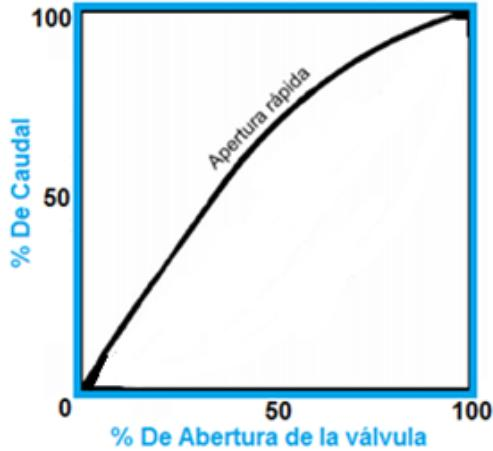
\includegraphics[scale=.50]{./Figures/funcion-valvula.jpeg}
\caption{Gráfica del caudal en función de la apertura de la válvula.}
\label{fig:grafica caudal vs. caudal}
\end{figure}

\subsection{Servomotor}
\label{subsec:Servomotor}
Para el control de la válvula fue necesario un motor que pueda producir un momento de 1 Nm o más. Para este proyecto, por cuestión de disponibilidad, se utilizó un motor paso a paso y un controlador cuyo modelos son 86HS85 y MA860H respectivamente.
El motor paso a paso de 8 hilos posee un torque nominal de 8,5 Nm, suficiente como para realizar movimientos de apertura parcial o total y cierre total de la carrera de dicha válvula, según las necesidades requeridas de caudal. 
El driver MA860H es un controlador para motores paso a paso compatibles con motores 86HS85 con las siguientes características principales:

\begin{enumerate}
	\item Permite ajustar la corriente que se dirige hacia el motor.
	\item Posibilita controlar al motor hasta en 200 micropasos.
	\item Frecuencia de entrada de tren de pulso hasta 300khz. 
	\item Corriente de salida hasta 7.2A.
	\item Entrada TTL compatible y ópticamente aislada.
	\item Soporta modos PUL / DIR y CW / CCW.
\end{enumerate}
El MA860H tiene dos conectores, el conector P1 para conexiones de señales de control y el conector P2 para conexiones de potencia y motor. 
\subsubsection{Configuraciones del conector P1}
PUL+,PUL-: Señal de pulso: esta entrada representa la señal de pulso, activa en cada flanco ascendente o descendente (para este trabajo se encuentra activo en flanco ascendente); 4-5V equivale a un pulso alto y 0-0.5V a un pulso bajo. Para una respuesta confiable, el ancho de pulso debe ser superior a 1,5 microssegundos. 
DIR+;DIR- : Señal DIR: esta señal tiene niveles de voltaje bajo / alto, que representan dos direcciones de rotación del motor. Para una respuesta de movimiento confiable, la señal DIR debe estar por delante de la señal PUL por lo menos 5 microsegundos. 4-5V cuando DIR-HIGH, 0-0.5V cuando DIR-LOW. 

ENA+;ENA-: Señal de Habilitación: esta señal se utiliza para habilitar/deshabilitar el controlador. Nivel alto (la señal de control NPN, PNP y las señales de control diferencial son por el contrario, es decir, nivel bajo para habilitar) para habilitar al controlador y nivel bajo para inhabilitar al controlador.
\subsubsection{Circuito interfaz del conector de señal de control (P1)}
El controlador MA860H puede aceptar entradas diferenciales y de un solo extremo (incluida la salida de colector abierto y PNP). El MA860H tiene 3 entradas lógicas aisladas ópticamente que están ubicadas en el conector P1 para aceptar señales de control del microcontrolador. Estas entradas están aisladas para minimizar o eliminar los ruidos eléctricos acoplados a las señales de control del variador. En la siguiente figura, se ilustra las conexiones a colector abierto.
\begin{figure}[h]
\centering
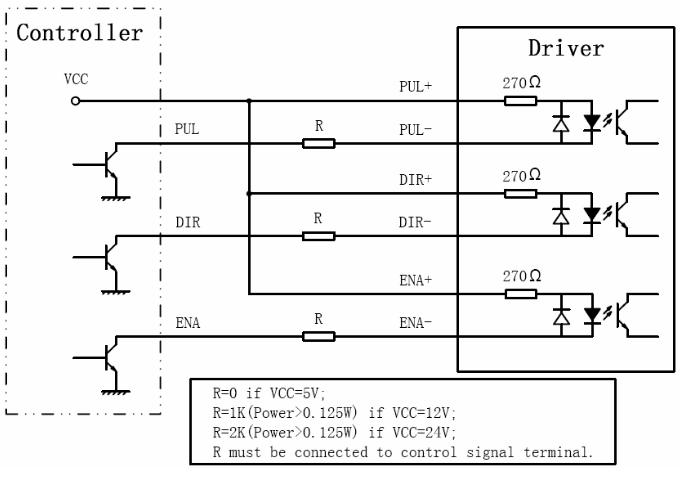
\includegraphics[scale=.65]{./Figures/circuitointerfaz-driver.jpeg}
\caption{Circuito Interfaz - conexiones de señales a colector abierto.}
\label{fig:circuito interfaz}
\end{figure}
Siguiendo las recomendaciones del fabricante relacionadas a la construcción del circuito interfaz entre el diver y el microcontrolador se diseñó y fabricó el circuito eléctrico que se muestra en la siguiente figura:

%Se puede agregar código o pseudocódigo dentro de un entorno lstlisting con el siguiente código:
%
%\begin{verbatim}
%\begin{lstlisting}[caption= "un epígrafe descriptivo"]
%	las líneas de código irían aquí...
%\end{lstlisting}
%\end{verbatim}
%
%A modo de ejemplo:
%
%\begin{lstlisting}[label=cod:vControl,caption=Pseudocódigo del lazo principal de control.]  % Start your code-block
%
%#define MAX_SENSOR_NUMBER 3
%#define MAX_ALARM_NUMBER  6
%#define MAX_ACTUATOR_NUMBER 6
%
%uint32_t sensorValue[MAX_SENSOR_NUMBER];		
%FunctionalState alarmControl[MAX_ALARM_NUMBER];	//ENABLE or DISABLE
%state_t alarmState[MAX_ALARM_NUMBER];						//ON or OFF
%state_t actuatorState[MAX_ACTUATOR_NUMBER];			//ON or OFF
%
%void vControl() {
%
%	initGlobalVariables();
%	
%	period = 500 ms;
%		
%	while(1) {
%
%		ticks = xTaskGetTickCount();
%		
%		updateSensors();
%		
%		updateAlarms();
%		
%		controlActuators();
%		
%		vTaskDelayUntil(&ticks, period);
%	}
%}
%\end{lstlisting}
%
%
%
